\chapter{Safe and Near Optimal Controller Synthesis for Stochastic hybrid Games}
  \label{ch:proposal} % In this part goes algorithm, case study and results
  In this part, we propose a case study \emph{Sthocastic Hybrid Solar Water
  Heating}, to apply our methodology, following the next procedure:
  \emph{System modelling} using physics criteria \cite{tsilingiris1996solar}. The use of
  mechanical concepts to have a \emph{stochastic
  hybrid game}. Some engineering assumptions either int the model and
  the configuration parameters are considered to facilate our analysis.
  A fundamental characteristic  of the model is the incorporation 
  of uncontrollable events for instance open the aperture valve or
  close it. 
  Secondly, our system interact with an environment, for this reason 
  we set some paremeters to get the environment conditions so as 
  understand the temporal data such as \emph{Irradiance}, \emph{external and 
  internal temperatures}, these perturbations are preprocessed to interact
  with our simulator \autoref{sec:casestudy}. To establish a safe sthocastic hybrid system, we start to compute patterns as
  \autoref{sec:safepatterncomputation} explains. It is important to bear in mind
  the uncontrollable events in our patterns computation to verify the safety
  in our system.
  Lastly, the computation of a near optimal controller consist of an 
  exhaustive exploration of different strategies in order to either
  minimize or maximize a cost function of a random variable in a 
  specific horizon and stochastic hybrid game, this computation is 
  using \textsc{uppaal stratego}. In control experiments we found that
  This methodology help to concatenate the two approaches implementing
  a toolbox for real time simulation in \textsc{python} \cite{larsen2016online}.
  \clearpage

  \section{Solar Water Heating Case study}
    \label{sec:casestudy}

    \begin{figure}[!hbt]
      


\tikzset{every picture/.style={line width=0.75pt}} %set default line width to 0.75pt        

\begin{tikzpicture}[x=0.75pt,y=0.75pt,yscale=-1,xscale=1]
%uncomment if require: \path (0,300); %set diagram left start at 0, and has height of 300

%Rounded Rect [id:dp3454362135099034] 
\draw   (203,113.4) .. controls (203,105.45) and (209.45,99) .. (217.4,99) -- (282.1,99) .. controls (290.05,99) and (296.5,105.45) .. (296.5,113.4) -- (296.5,156.6) .. controls (296.5,164.55) and (290.05,171) .. (282.1,171) -- (217.4,171) .. controls (209.45,171) and (203,164.55) .. (203,156.6) -- cycle ;
%Straight Lines [id:da8670184653139519] 
\draw    (232.5,128) -- (175.5,128.97) ;
\draw [shift={(173.5,129)}, rotate = 359.03] [color={rgb, 255:red, 0; green, 0; blue, 0 }  ][line width=0.75]    (10.93,-3.29) .. controls (6.95,-1.4) and (3.31,-0.3) .. (0,0) .. controls (3.31,0.3) and (6.95,1.4) .. (10.93,3.29)   ;

%Image [id:dp1573774251550818] 
\draw (329.75,151.22) node  {\includegraphics[width=391.13pt,height=232.5pt]{5.png}};
%Straight Lines [id:da756821456781489] 
\draw    (360.5,151.22) -- (442.5,150.24) ;
\draw [shift={(444.5,150.22)}, rotate = 539.3199999999999] [color={rgb, 255:red, 0; green, 0; blue, 0 }  ][line width=0.75]    (10.93,-3.29) .. controls (6.95,-1.4) and (3.31,-0.3) .. (0,0) .. controls (3.31,0.3) and (6.95,1.4) .. (10.93,3.29)   ;


%Straight Lines [id:da9580285561891552] 
\draw    (228.5,102.22) -- (302.5,101.24) ;
\draw [shift={(304.5,101.22)}, rotate = 539.25] [color={rgb, 255:red, 0; green, 0; blue, 0 }  ][line width=0.75]    (10.93,-3.29) .. controls (6.95,-1.4) and (3.31,-0.3) .. (0,0) .. controls (3.31,0.3) and (6.95,1.4) .. (10.93,3.29)   ;

%Straight Lines [id:da9281060785864365] 
\draw    (389.5,67.22) -- (430.5,67.22) ;
\draw [shift={(432.5,67.22)}, rotate = 180] [color={rgb, 255:red, 0; green, 0; blue, 0 }  ][line width=0.75]    (10.93,-3.29) .. controls (6.95,-1.4) and (3.31,-0.3) .. (0,0) .. controls (3.31,0.3) and (6.95,1.4) .. (10.93,3.29)   ;

%Straight Lines [id:da47053369422446445] 
\draw    (261.5,79.22) -- (294.5,79.22) ;
\draw [shift={(296.5,79.22)}, rotate = 180] [color={rgb, 255:red, 0; green, 0; blue, 0 }  ][line width=0.75]    (10.93,-3.29) .. controls (6.95,-1.4) and (3.31,-0.3) .. (0,0) .. controls (3.31,0.3) and (6.95,1.4) .. (10.93,3.29)   ;

%Shape: Circle [id:dp11314595015500317] 
\draw  [color={rgb, 255:red, 0; green, 0; blue, 0 }  ,draw opacity=1 ][fill={rgb, 255:red, 155; green, 155; blue, 155 }  ,fill opacity=1 ] (532.5,92.75) .. controls (532.5,88.19) and (536.19,84.5) .. (540.75,84.5) .. controls (545.31,84.5) and (549,88.19) .. (549,92.75) .. controls (549,97.31) and (545.31,101) .. (540.75,101) .. controls (536.19,101) and (532.5,97.31) .. (532.5,92.75) -- cycle ;

% Text Node
\draw (463,133) node   {$kA_{t}( T_{cont} -T_{env})$};
% Text Node
\draw (193,97) node   {$A_{c}( I_{env})$};
% Text Node
\draw (474,48) node   {$m( T_{cont} -T_{in})$};
% Text Node
\draw (339,116) node   {$T_{cont}$};
% Text Node
\draw (568,89) node   {$T_{env}$};
% Text Node
\draw (539,278) node   {$T_{in}$};
% Text Node
\draw (276,60) node   {$P_{aux}$};
% Text Node
\draw (540,217) node   {$T_{cont}$};


\end{tikzpicture}

      \caption{Solar Water Heating diagram}
      \label{fig:casestudy}
    \end{figure}

    \subsection{data analysis}
      \textbf{Stochastic events as historical data}. In practice
      we notice unpredictable discrete events which can perturbate a dynamical 
      system, these stochastic discrete perturbations we call uncontrallable actions and 
      is managed using a stochastic approach and machine learning to optimize
      the behaviour. Generate this actions with a realist criteria for our case study 
      we choose three gaussian distributions with $\mu_1 = 7h$, $\mu_2 = 12h$ and $\mu_3 = 19h$
      and $\sigma_1=12,\sigma_2=15, \sigma_3=10$ respectively. Finally we add 
      a uniform distribution around the day.
      \begin{figure}[!hbt]      
        \includegraphics[width=1.2\linewidth]{images/uncontrollable}      
        \captionof{figure}{State changes of valves along the day.}
        \label{fig:uncontrollable}
      \end{figure}

      \clearpage

      \textbf{Solaris Data and preprocessing} The data collected is from 
      spain solaris, which consist of a set of environment features such as
      environment temperature and irradiance that would be useful for the 
      simulation. However, we preprocess the data for our purpose such us
      modify the time step from 15 minutes to 1 minute trough interpolation.
      \begin{figure}[!hbt]
        \includegraphics[width=1.2\linewidth]{images/solaris2}
        \captionof{figure}{Weather time series, irradiance and temperature }
      \end{figure}
      % \begin{minipage}{\linewidth}
      %     \begin{center}  
      %         \includegraphics[width=1.2\linewidth]{images/solaris2}
      %         \captionof{figure}{An example image not including a Wombat}
      %     \end{center}
      % \end{minipage}
      
      \textbf{Prediction Data}.
      To integrate a model predictive controller approach we had to implement 
      a forecaster in real time in order to get a sequence of environment data
      on future which will be used to control future states an get the correct
      patterns on present. \textsc{arima} state model is used with a realtime 
      pivot .. bla bla .
      \begin{minipage}{\linewidth}
        \begin{center}
            \includegraphics[width=0.7\linewidth]{images/prediction}
            \captionof{figure}{An example of prediction using \textsc{arima} forecaster}
            \label{prediction_environment}
        \end{center}
      \end{minipage}
      \clearpage
  
    % % equation description
    % The energy inside of the container is calculated as a control volume, an abstract
    % region which experiment power input and output, doing a energy balance is obtained
    % the dynamical either volumen or temperature as described in \ref{energy-balance}
    % and \ref{volume-balance}.
    % \begin{equation} 
    % §    \factorheat\mcont(t)\frac{d}{dt}\tcont =  A_c\irradiance + \haux - v\factorheat \flowin (\tcont-\tin) -   k_c A_t (\tcont-\tenv) + rQ
    %     \label{energy-balance}
    % \end{equation}
    % \begin{equation}
    %     \frac{d}{dt}\mcont(t) =  \rho \frac{d}{dt}\vcont = \rho (pV_{min} - \vcont); \quad
    %     \label{volume-balance}
    % \end{equation}

    % table 
      \begin{table}[hbt!]
      \begin{tabular}{ |p{2cm}||p{6cm}|p{2cm}|p{2cm}|  }
          \hline
          \multicolumn{4}{|c|}{States} \\
          \hline
          Variable& Description &Initial Value&Units\\    
          \hline    
          E & Energy consumption  & 0.0 & \si{\joule} \\
          V & Container Volumen  & 0.13 &\si{\metre^3}\\
          T & Container Temperature & 50.0 & \si{\degreeCelsius}  \\            
          \hline
          \multicolumn{4}{|c|}{Constants} \\
          \hline    
          Variable& Description & Value & Units\\        
          \hline
          \factorheat & The factor heat of the water in   & 4186&\si{\joule\per\degreeCelsius\per\kilogram}\\
          \flowin & Mass flow rate input/output  & 0.1  &\si{\kilogram\per\second}\\
          \mcont & the mass of the container in & 100 & \si{\kilogram} \\    
          $A_c$ & Area of colector in & 1 & \si{\metre^2} \\
          $A_t$ & Area of total of surface in & 5.56 & \si{\metre^2} \\
          $k_c$ & Conduction coeficient & 16 & \si{\watt\per\metre\per\degreeCelsius} \\
          $\haux$ & Auxiliary heat power in & 1000 & \si{\watt} \\    
          \hline
          \multicolumn{4}{|c|}{Input values} \\
          \hline    
          Variable& Description &  \multicolumn{2}{|c|}{Space values}\\
          \hline
          $v$ & Controllable action to release water & \multicolumn{2}{|c|}{$\left\lbrace 0,1 \right\rbrace$} \\
          \hline
          $r$ & Controllable action to heat & \multicolumn{2}{|c|}{$\left\lbrace 0,1 \right\rbrace$}\\
          \hline
          $p$ & Uncontrollable action to change capacity water & \multicolumn{2}{|c|}{$\left\lbrace 1,2,3 \right\rbrace$}\\
          \hline         
          \multicolumn{4}{|c|}{Disturbances} \\
          \hline
          Variable& Description & Range&Units\\
          \hline
          $\tin$ & the temperature of water input/output in & $[20-25]$ & \si{\degreeCelsius} \\
          $\irradiance$ & the irradiance in & $[0-920]$ & \si{\watt\per\square\metre}    \\
          $\tenv$ & the outside temperature in & $[0-16.5]$ & \si{\degreeCelsius} \\
          \hline
      \end{tabular}
      \caption{Parameter values are used to compute $c_1,c_2, c_3$ and $c_4$.}
      \label{data-table}
      \end{table}
      \clearpage
    \subsection{Hybrid Solar Water Heating as a Sthocastic Hybrid Game}.
    The hybrid solar water heating scenario with 12 modes of operations is
    defined  like this: $\mathcal{G}_{n,m} = (\mathcal{C,U,X,F},\delta)$, 
    where the controller $\mathcal{C}$ has a finite set of controllable modes,
    given by resistance state ${r \in \mathbb{B}}$ and piston position $p \in 
    \left\lbrace1,2,3\right\rbrace $. The environment $\mathcal{U}$ has a finite  
    set of uncontrollable modes $v \in \mathbb{B} $, that means the valve state 
    for opening/closing water aperture. \hlc{We assume that $\mathcal{U}$ given
    $\delta$ can switch among modes with equal probability at every period}. 
    The state variables in $\mathcal{X}$ are given by $\left\lbrace 
    T,E,V \right\rbrace $, container temperature, energy used and container 
    volumen respectively.

    Given the container temparature and volume, a controllable modes $r \in \mathbb{B}$
    and $p \in \left\lbrace1,2,3\right\rbrace $ and uncontrollable mode
    $v \in \mathbb{B} $ and a time delay $\tau$ \autoref{fig:casestudy}.

    \begin{equation}
      \begin{aligned}
        \frac{d}{dt}\tcont = \frac{1}{V(t)} [ -\constone(\tcont-\tenv)
        - v \consttwo(\tcont-\tin) \\
        - f \constthree(pV_{min} - \vcont)(\tcont-\tin)
        + \constfour\irradiance+ 
        r \constfive ]
      \end{aligned}
      \label{temperature-equation}
    \end{equation}

    \begin{equation}
    \frac{d}{dt}\vcont = pV_{min} - \vcont; \quad
    \label{volume-equation}
    \end{equation}

    \begin{equation} 
    \frac{d}{dt}E_{used} =  r \constthree ;
    \label{Energy-equation}
    \end{equation}

    The equation \ref{temperature-equation} has some constants $\left\lbrace 
    \constone, \consttwo, \constthree, \constfour \right\rbrace $ this
    parameters are computed with the parameteres defines in table \ref{data-table} 
    and equal to $\left\lbrace 2.44e^{-5},  4.77e^{-6}, 0.0024, 0.01 \right\rbrace$ respectively.
    Another important variable to consider is $f$, which
    means the transition between event $p$ and $p'$ which create a term that affect the total energy
    \autoref{temperature-equation}, this term measure the changes of energy when the
    piston is in expansion thus, the water entrance and the container temperature decrement
    so as the increment of the volume, or contraction which cause water dispense 
    the loss of total energy decreasing the volumen but not the container temperature.
    $p < p' \rightarrow f' == 1$, which means a piston expansion otherwise a piston contraction 
    $p \geqslant p' \rightarrow f' == 0$, in initial conditions we set $f == 0$.
    
    According to our case study we find some transisions such as $\gamma_2 \xrightarrow{\tau} \gamma_{0} $,
    $\gamma_3 \xrightarrow{\tau} \gamma_{0} $, $\gamma_2 \xrightarrow{\tau} \gamma_{1} $,
    $\gamma_3 \xrightarrow{\tau} \gamma_{0} $ so as $\gamma_6 \xrightarrow{\tau} \gamma_{3} $,
    $\gamma_7 \xrightarrow{\tau} \gamma_{3} $, $\gamma_6 \xrightarrow{\tau} \gamma_{5} $,
    $\gamma_7 \xrightarrow{\tau} \gamma_{5} $
    \clearpage

    \begin{figure}[!hbt]
      

\tikzset{every picture/.style={line width=0.75pt}} %set default line width to 0.75pt        

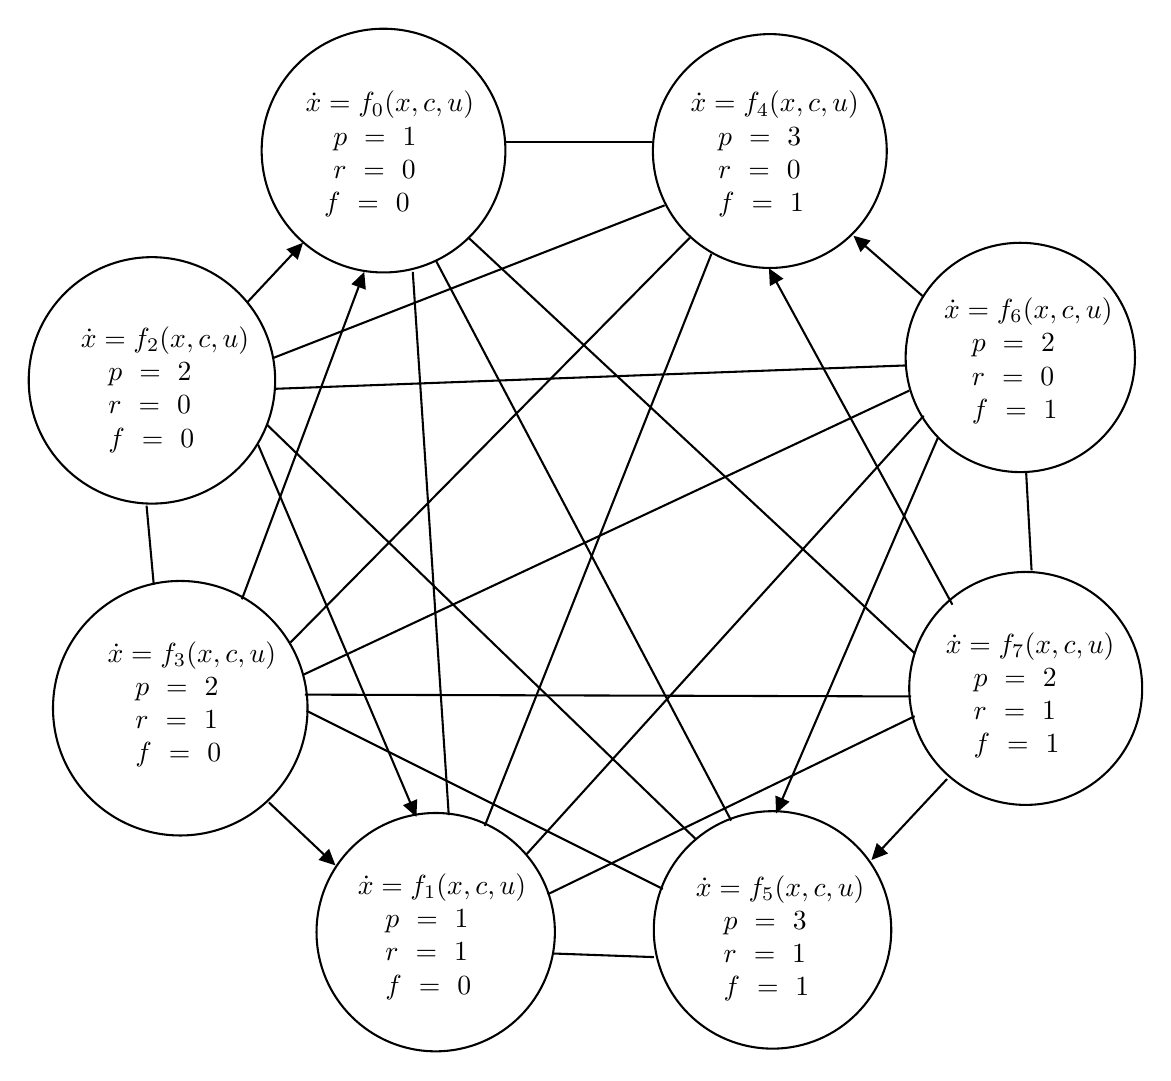
\begin{tikzpicture}[x=0.65pt,y=0.65pt,yscale=-1,xscale=1]
%uncomment if require: \path (0,869); %set diagram left start at 0, and has height of 869

%Shape: Circle [id:dp8105865911695849] 
\draw   (382.5,274.5) .. controls (382.5,236.67) and (413.17,206) .. (451,206) .. controls (488.83,206) and (519.5,236.67) .. (519.5,274.5) .. controls (519.5,312.33) and (488.83,343) .. (451,343) .. controls (413.17,343) and (382.5,312.33) .. (382.5,274.5) -- cycle ;
%Shape: Circle [id:dp4238655727754186] 
\draw   (396,456.75) .. controls (396,417.68) and (427.68,386) .. (466.75,386) .. controls (505.82,386) and (537.5,417.68) .. (537.5,456.75) .. controls (537.5,495.82) and (505.82,527.5) .. (466.75,527.5) .. controls (427.68,527.5) and (396,495.82) .. (396,456.75) -- cycle ;
%Shape: Circle [id:dp2933944994958515] 
\draw   (512,146.75) .. controls (512,109.33) and (542.33,79) .. (579.75,79) .. controls (617.17,79) and (647.5,109.33) .. (647.5,146.75) .. controls (647.5,184.17) and (617.17,214.5) .. (579.75,214.5) .. controls (542.33,214.5) and (512,184.17) .. (512,146.75) -- cycle ;
%Shape: Circle [id:dp9366456554811557] 
\draw   (542.5,581.25) .. controls (542.5,544.66) and (572.16,515) .. (608.75,515) .. controls (645.34,515) and (675,544.66) .. (675,581.25) .. controls (675,617.84) and (645.34,647.5) .. (608.75,647.5) .. controls (572.16,647.5) and (542.5,617.84) .. (542.5,581.25) -- cycle ;
%Shape: Circle [id:dp7320262061476854] 
\draw   (729.5,147) .. controls (729.5,111.1) and (758.6,82) .. (794.5,82) .. controls (830.4,82) and (859.5,111.1) .. (859.5,147) .. controls (859.5,182.9) and (830.4,212) .. (794.5,212) .. controls (758.6,212) and (729.5,182.9) .. (729.5,147) -- cycle ;
%Shape: Circle [id:dp08196792261757313] 
\draw   (730,580) .. controls (730,543.55) and (759.55,514) .. (796,514) .. controls (832.45,514) and (862,543.55) .. (862,580) .. controls (862,616.45) and (832.45,646) .. (796,646) .. controls (759.55,646) and (730,616.45) .. (730,580) -- cycle ;
%Shape: Circle [id:dp2726927054913544] 
\draw   (870,261.75) .. controls (870,226.54) and (898.54,198) .. (933.75,198) .. controls (968.96,198) and (997.5,226.54) .. (997.5,261.75) .. controls (997.5,296.96) and (968.96,325.5) .. (933.75,325.5) .. controls (898.54,325.5) and (870,296.96) .. (870,261.75) -- cycle ;
%Shape: Circle [id:dp447834466431017] 
\draw   (872,445.75) .. controls (872,409.99) and (900.99,381) .. (936.75,381) .. controls (972.51,381) and (1001.5,409.99) .. (1001.5,445.75) .. controls (1001.5,481.51) and (972.51,510.5) .. (936.75,510.5) .. controls (900.99,510.5) and (872,481.51) .. (872,445.75) -- cycle ;
%Straight Lines [id:da771329734195769] 
\draw    (504.01,231.11) -- (532.95,200.19) ;
\draw [shift={(535,198)}, rotate = 493.1] [fill={rgb, 255:red, 0; green, 0; blue, 0 }  ][line width=0.08]  [draw opacity=0] (8.93,-4.29) -- (0,0) -- (8.93,4.29) -- cycle    ;
%Straight Lines [id:da24943983750644705] 
\draw    (647.01,142.11) -- (729.01,142.11) ;
%Straight Lines [id:da9374471528095312] 
\draw    (843.28,196.08) -- (880.01,228.11) ;
\draw [shift={(841.01,194.11)}, rotate = 41.08] [fill={rgb, 255:red, 0; green, 0; blue, 0 }  ][line width=0.08]  [draw opacity=0] (8.93,-4.29) -- (0,0) -- (8.93,4.29) -- cycle    ;
%Straight Lines [id:da20228861715808955] 
\draw    (937.01,326.11) -- (940.01,380.11) ;
%Straight Lines [id:da1309980038885339] 
\draw    (730.01,595.11) -- (674.01,593.11) ;
%Straight Lines [id:da8387653364416086] 
\draw    (893.01,496.11) -- (853.06,538.91) ;
\draw [shift={(851.01,541.11)}, rotate = 313.03] [fill={rgb, 255:red, 0; green, 0; blue, 0 }  ][line width=0.08]  [draw opacity=0] (8.93,-4.29) -- (0,0) -- (8.93,4.29) -- cycle    ;
%Straight Lines [id:da15505665307834682] 
\draw    (550.83,542.05) -- (516.01,509.11) ;
\draw [shift={(553.01,544.11)}, rotate = 223.41] [fill={rgb, 255:red, 0; green, 0; blue, 0 }  ][line width=0.08]  [draw opacity=0] (8.93,-4.29) -- (0,0) -- (8.93,4.29) -- cycle    ;
%Straight Lines [id:da9785106227459619] 
\draw    (452.01,388.11) -- (448.01,344.11) ;
%Straight Lines [id:da40579582190774643] 
\draw    (795.45,214.83) -- (896.01,399.2) ;
\draw [shift={(794.01,212.2)}, rotate = 61.39] [fill={rgb, 255:red, 0; green, 0; blue, 0 }  ][line width=0.08]  [draw opacity=0] (8.93,-4.29) -- (0,0) -- (8.93,4.29) -- cycle    ;
%Straight Lines [id:da9504222588958726] 
\draw    (888.01,306.2) -- (799.2,512.44) ;
\draw [shift={(798.01,515.2)}, rotate = 293.3] [fill={rgb, 255:red, 0; green, 0; blue, 0 }  ][line width=0.08]  [draw opacity=0] (8.93,-4.29) -- (0,0) -- (8.93,4.29) -- cycle    ;
%Straight Lines [id:da4817256852969489] 
\draw    (510.01,310.2) -- (596.84,514.44) ;
\draw [shift={(598.01,517.2)}, rotate = 246.97] [fill={rgb, 255:red, 0; green, 0; blue, 0 }  ][line width=0.08]  [draw opacity=0] (8.93,-4.29) -- (0,0) -- (8.93,4.29) -- cycle    ;
%Straight Lines [id:da5197840649707755] 
\draw    (567.96,217.01) -- (501.01,396.2) ;
\draw [shift={(569.01,214.2)}, rotate = 110.49] [fill={rgb, 255:red, 0; green, 0; blue, 0 }  ][line width=0.08]  [draw opacity=0] (8.93,-4.29) -- (0,0) -- (8.93,4.29) -- cycle    ;
%Straight Lines [id:da6155672485715638] 
\draw    (519.01,279.2) -- (870.01,266.2) ;
%Straight Lines [id:da5361536697962814] 
\draw    (518.01,262.2) -- (736.01,177.2) ;
%Straight Lines [id:da7329803706341473] 
\draw    (536.01,449.2) -- (873.01,450.2) ;
%Straight Lines [id:da47359936905090594] 
\draw    (659.01,538.2) -- (880.01,294.2) ;
%Straight Lines [id:da5004090611197451] 
\draw    (762.01,204.2) -- (636.01,522.2) ;
%Straight Lines [id:da8612879134092823] 
\draw    (596.01,214.2) -- (616.01,516.2) ;
%Straight Lines [id:da26459344362918436] 
\draw    (535.01,438.2) -- (872.01,280.2) ;
%Straight Lines [id:da8834205218815725] 
\draw    (537.01,458.2) -- (735.01,557.2) ;
%Straight Lines [id:da2941468624363204] 
\draw    (528.01,420.2) -- (750.01,195.2) ;
%Straight Lines [id:da9095983178937885] 
\draw    (515.01,299.2) -- (753.01,529.2) ;
%Straight Lines [id:da668275173400011] 
\draw    (627.01,195.2) -- (875.01,426.2) ;
%Straight Lines [id:da943066290095641] 
\draw    (609.01,208.2) -- (773.01,519.2) ;
%Straight Lines [id:da14407547098091467] 
\draw    (671.01,560.2) -- (875.01,461.2) ;

% Text Node
\draw (458.25,280.25) node    {$ \begin{array}{l}
\dot{x} =f_{2}( x,c,u)\\
\ \ \ p\ =\ 2\\
\ \ \ r\ =\ 0\\
\ \ \ f\ =\ 0
\end{array}$};
% Text Node
\draw (473.25,455.25) node    {$ \begin{array}{l}
\dot{x} =f_{3}( x,c,u)\\
\ \ \ p\ =\ 2\\
\ \ \ r\ =\ 1\\
\ \ \ f\ =\ 0
\end{array}$};
% Text Node
\draw (797.25,149.25) node    {$ \begin{array}{l}
\dot{x} =f_{4}( x,c,u)\\
\ \ \ p\ =\ 3\\
\ \ \ r\ =\ 0\\
\ \ \ f\ =\ 1
\end{array}$};
% Text Node
\draw (800.25,585.25) node    {$ \begin{array}{l}
\dot{x} =f_{5}( x,c,u)\\
\ \ \ p\ =\ 3\\
\ \ \ r\ =\ 1\\
\ \ \ f\ =\ 1
\end{array}$};
% Text Node
\draw (583.25,149.25) node    {$ \begin{array}{l}
\dot{x} =f_{0}( x,c,u)\\
\ \ \ p\ =\ 1\\
\ \ \ r\ =\ 0\\
\ \ f\ =\ 0
\end{array}$};
% Text Node
\draw (612.25,584.25) node    {$ \begin{array}{l}
\dot{x} =f_{1}( x,c,u)\\
\ \ \ p\ =\ 1\\
\ \ \ r\ =\ 1\\
\ \ \ f\ =\ 0
\end{array}$};
% Text Node
\draw (938.25,264.25) node    {$ \begin{array}{l}
\dot{x} =f_{6}( x,c,u)\\
\ \ \ p\ =\ 2\\
\ \ \ r\ =\ 0\\
\ \ \ f\ =\ 1
\end{array}$};
% Text Node
\draw (939.25,450.25) node    {$ \begin{array}{l}
\dot{x} =f_{7}( x,c,u)\\
\ \ \ p\ =\ 2\\
\ \ \ r\ =\ 1\ \\
\ \ \ f\ =\ 1
\end{array}$};


\end{tikzpicture}

      \caption{Automaton with forbidden transitions because of the addition of a 
      discrete variable \emph{f} which facilate the system modelling in cases such
       as piston expansion and compression.}
      \label{fig:automaton}
    \end{figure}

    Finally we set as controllable actions $c = (p,r,f) \in \lbrace 1,2,3 \rbrace \times 
    \lbrace 0,1 \rbrace \times \lbrace 0,1 \rbrace $ and uncontrollable actions 
    \hlc{ $u = \sum_{i=0}^{3} p_{i}(t)$, $p_1(t)$ }as shown at \autoref{fig:uncontrollable}.    
    \clearpage 
    \section{Experiments: }
    \subsection{Patterns computation}
    To establish a safe sthocastic hybrid system,
    we start to compute patterns as \autoref{sec:safepatterncomputation} 
    explains. It is important to bear in mind that the stochastic events 
    shall not be considered as discrete state but as interval, \hlc{in other 
    words the sthocastic action will be composed by lower case when valve
    is close doing the loss energy as zero and the higher case when valve 
    is open doing loss energy due to water dispense}. Safe patterns are 
    computed and associated to zonotopes,which are regions where patterns
    verify the next: Given $D = 20, K = 3$ and by constructing a law 
    $\sigma(.)$, such that for all $x_o \in R$, and under the unknown 
    bounded perturbation $d$, there exists $\pi = \sigma(.) \in U^k$ for
     some $k$ such that:
    \begin{center}
      $x(t_0 + k\tau; t_0,x_0,d,\pi) \in R$ \\
      $\forall t\in  \lbrack t_0, t_0+k\tau\rbrack, x(t; t_0,x_0,d,\pi)
       \in S $  \\
      $\forall t\in  \lbrack t_0, t_0+k\tau\rbrack, x(t; t_0,x_0,d,\pi)
       \not\in B$
    \end{center}
    Such a law permits to perform a safe control guaranteeing limits for each
    action in each step conditioning a safe sequence of modes called 
    \emph{pattern}. We configurate $R = \begin{bmatrix} 40 & 70 \\ 0.1 & 0.2
    \end{bmatrix}$, $S = \begin{bmatrix} 30 & 80 \\ 0.09 & 0.31 \end{bmatrix}$,
    $W = \begin{bmatrix} 40 & 70 \\ 0.1 & 0.2 \end{bmatrix}$,
    $B = \begin{bmatrix} 0 & 0 \\ 0 & 0 \end{bmatrix}$, after to run the 
    
    \textbf{Proposition 1.} \emph{
      Algorithm Decomposition with input (R,R,S,B,D,K) returns, when it successfully 
      terminates, a decomposition $\lbrace V_i, \pi_i \rbrace_{i \in I}$ 
      of $R$ which solves Problem 1.
    }    
    \clearpage

    There are forbidden transitions in the automaton, for this reason we 
    modify the algorithm which only permit to evaluate allowed transitions, otherwise
    the algorihtm ignore the mode exploring other modes to complete the pattern.
    
    \begin{algorithm}
      \caption{Find Pattern with forbidden transitions}\label{euclid}
      \begin{algorithmic}[1]
        \Procedure{FindPattern}{$W,R,S,B,K$}\Comment{List of set of patterns} \\
          \textbf{Input:} A box $W$, a box $R$,
          a box $S$, a box $B$, a length $K$ of input pattern\\
          \textbf{Output:} $<\prod,True> or <_,False>$ \\
          $\mathcal{S}= \lbrace \emptyset \rbrace$ \\
          $\mathcal{L}= \lbrace (W,W,\emptyset) \rbrace$
          \While{$\mathcal{L} \neq \emptyset$}
            \State $e_{current} = takeHead(\mathcal{L})$
            \For{$i \in U$}:
              \If {$Pair(l,i) = False $}\Comment{$l$ is the current mode}
                \State \textbf{continue}\Comment{Not considered transition $l,i$}
              \EndIf
              \label{alg:filter_transitions}
              \If {$ Post_{i}(e_{current}.Y_{current}) \subseteq R$ \textbf{and} $Tube_{i}(e_{current}.Y_{current}) \cup B = \emptyset $ \textbf{and} $Tube_{i}(e_{current}.Y_{current}) \cup B \subseteq S $ }
                \State putTail($\mathcal{S}e_{current}.\prod + i$)
              \Else
                \If{$ Tube_{i}(e_{current}.Y_{current}) \cap B \neq \emptyset $ \textbf{or} $ Tube_{i}(e_{current}.Y_{current}) \nsubseteq S $}
                  \State discard $e_{current}$
                \EndIf
                \If{$ Tube_{i}(e_{current}.Y_{current}) \cap B = \emptyset $ \textbf{and} $ Tube_{i}(e_{current}.Y_{current}) \subseteq S $}
                  \If {$Length(\prod)+1<K$}
                    \State putTail$(\mathcal{L},(e_{current}.Y_{init}.Post_{i}(e_{current}.Y_{current}),e_{current}.\prod+i))$
                  \EndIf              
                \EndIf
              \EndIf
            \EndFor          
          \EndWhile
          \State \textbf{return} $<_,False>$ \Comment{if no solution is found, or $<\prod,True>$, $\prod$ beaing any pattern validated in $Solution$.}
        \EndProcedure    
      \end{algorithmic}
    \end{algorithm}
  
    The algorithm find pattern second version on \cite{le2017improved} 
    is improved filtering invalid transition in the line \ref{alg:filter_transitions}.     
    % $R = \lbrack 40,70; 0.1,0.2 \rbrack $
    \begin{figure}[!hbt]
      \begin{center}
          

\tikzset{every picture/.style={line width=0.75pt}} %set default line width to 0.75pt        

\begin{tikzpicture}[x=0.75pt,y=0.75pt,yscale=-1,xscale=1]
%uncomment if require: \path (0,310); %set diagram left start at 0, and has height of 310

%Image [id:dp5662256713421685] 
\draw (319,152) node  {\includegraphics[width=274.5pt,height=246pt]{content/sources/safe_post_pattern.png}};

% Text Node
\draw (218,194) node [anchor=north west][inner sep=0.75pt]   [align=left] {$\displaystyle R$};
% Text Node
\draw (206,240) node [anchor=north west][inner sep=0.75pt]   [align=left] {$\displaystyle S$};
% Text Node
\draw (335,150) node [anchor=north west][inner sep=0.75pt]   [align=left] {$\pi _{1} =( 1,3,0)$};
% Text Node
\draw (381,71) node [anchor=north west][inner sep=0.75pt]   [align=left] {$\pi _{2} =( 5,0)$};
% Text Node
\draw (228,96) node [anchor=north west][inner sep=0.75pt]   [align=left] {$\pi _{3} =( 4,0)$};

\end{tikzpicture}

          \caption{Simulation for the firsts three patterns}
      \end{center}
    \end{figure}
    
    % caption simulate the first 3 patterns randomly  acording to the right zonotope.     
    
    % AJA
    \textsc{python simulator}. We implement a \emph{toolbox} which support
    sthocastic hybrid models $\mathcal{G}_{n,m}$ and controllers $\mathcal{C}$. The models works with seasonal data 
    disturbances for this reason we incorporate modules to preprocess the data.
    \textbf{Simulation} In the initial step of the Model predictive algorithm to control,
    we use the first pattern corresponding to the current zonotope. In the subsequent 
    iterations e use the \textsc{stratego} to find a near optimal strategy from a selected
    set of safe patterns as show \ref{strategotemplate}. It is very important to bear in mind 
    the way of model predictive controler operate which is an asynchrnous call 
    before finish the last mode in the current pattern, sending to \textsc{stratego}
    the current dynamical states such as \emph{mode, volume, temperature} and so on with the
    corresponding environment predictions \ref{prediction_environment}.
    After the near optimal pattern computation for stochastic hybrid game 
    by \textsc{stratego} the process repeat.

    \textsc{uppaal stratego}. 

    \textbf{Learning strategies for PTMPDs}
    The algorithm used to learn will generate an approximation of the optimal strategy.
    The algorithm has five main phases, and one optional. All these can be seen 
    in \textsc{fig} . We will now shortly each of these steps. In the following 
    sections. 

    check learning optimal schedullign for time uncertain cet
    \textbf{Simuation}
    \textbf{Filtering}
    \textbf{Learning}
    \textbf{Determinization}
    \textbf{Evaluation}

    uncontrollable action si defined in a interval [min, max] at the moment to run 
    the find pattern. 

    \textbf{add this part}
    add the pseudocode about the methodoloy pattern and near optimal.

    \textbf{add the uppaal template}
    in this part add a figure with the template and describe it.


    \clearpage

    \subsection{Near optimal Experiments}
    Regarding our experiments, we have two major components: a simulator 
    written in  \textsc{Python} and a number of controllers, including 
    the ones produced by \textsc{uppaal stratego}. The simulator implements
    a solar water heating as stochastic hybrid game $\mathcal{G}_{n,m}$. For our 
    experiments, in the simulator we fix a time horizon \emph{H} of 75 minutes
    with a period \emph{P} of 5 minutes. As in the real house, every 
    5 minutes, the simulator outputs the current container values such as
    temperature \emph{T}, volume \emph{V}, energy \emph{E}, mode and predicted 
    environment data Subsequently, the controller inputs the control actions 
    such as resistor \emph{r}, piston \emph{p} which are used by the simulator  
    for the next 5 minutes. The house has a desired temperature $T^g$ and alpha
    parameters which denotes the importance to minimize either target or 
    energy consumption. Our goal is to optimize the comfort for the water 
    consumption reducing the energy consumption. To define 
    this cost function subject to controller (strategy) $\sigma$ and 
    $\mathcal{G}_{n,m}$ of the form $\pi = \gamma_0 \xrightarrow{t_{1}} 
    \gamma_1 \xrightarrow{t_{2}} ... \xrightarrow{t_{k-1}} 
    \gamma_{k-1} \xrightarrow{t_{k}} \gamma_{k}$ where $k = H/P$ is the 
    number of control steps in the run $\pi$. Let $T_{i}(\gamma_j)$ denote
    the container temperature $T_i$ at configuration $\gamma_j$. Then the 
    cost function is defined by

    \begin{equation}
      \begin{aligned}
          cost(\pi) = \alpha(E) + (1-\alpha)(T-T_g)
      \end{aligned}
    \end{equation}

    In our experiments, we evaluate a number of different controllers. The 
    simulator uses the cost function to compare the different
    controllers.

    \textbf{Controllers}. In the following we introduce a number of controllers
    which we use in out experiments. We present the current controller operating
    in the house, two controllers proposed by engineers and the controllers 
    synthetized using online synthesis and \textsc{uppaal-stratego}.

    % \emph{Bang-Bang Controller}. The bang-bang controller is currently running
    % in the physical house and after each reading of container temperature $T$,
    % it simply switch the resistor $ON$ of container where $T < T^g$ and leaves 
    % the remaining switch $OFF$.

    \emph{Safe Greddy Controller with Patterns}. 
    The greddy controller explore pattern by pattern and is chosen those which minimize
    the cost function, due to the use of complete patterns it guarantee a safe 
    behaviour and is optimize without consider the uncontrollable action 
    valve thus it could be optimize even more from a sthocastic approach.

    \emph{Statego Online Controller}.
    The Figure environment "floats" to find an optimal position on the page
    . When you begin a figure, you can use the options [htbp!] to specify whether 
    the figure should go "here", the "top" of this page, the "bottom" of this page,
     or a special "page" reserved for floats. LaTeX, in its infinite wisdom,
      will sometimes prevent you from putting a figure in an "ugly" place, 
      but you can (sort of) override its decision using the "!" option. 
      When you haven't used any option, the environment assumes that you
       provided [tbp], and it's choosing to put the figure at the top of
        the page, above where your section goes.

        
    \begin{minipage}{\linewidth}
      \begin{center}
          \includegraphics[width=0.8\linewidth]{images/controllers}
          \captionof{figure}{Container temparature comparison between greedy controller with 
          uppaal stratego controller, both approaches are safe.}
      \end{center}
      \label{uncontrollableactions}
    \end{minipage}

    \begin{minipage}{\linewidth}
      \begin{center}
          \includegraphics[width=1.0\linewidth]{images/automaton_uppaal}
          \captionof{figure}{Template of the safe an near optimal algorithm}
      \end{center}
      \label{strategotemplate}
    \end{minipage}
    We can observe an algorithm that run on \textsc{stratego}, this template 
    is adapted to find near optimal strategies for stochastic hybrid games, 
    \hlc{some heuristics are running for an exhaustive stochastic exploration} and
    reinforcement learning is used to 

    \emph{Safe and Near Optimal Controller}.


    \textbf{Evaluation Scenarios}

    \textbf{Controller Evaluation}

